\section{Generalization Analysis}

\begin{tcolorbox}
\textbf{Q1:} From the perspective of stability, how does the introduction of the weight decay fundamentally reshape the stability bound of the learning algorithm? To maintain optimal system performance, what dependencies must other hyperparameters exhibit? 
\end{tcolorbox}

In fact, \citet{10.5555/2986916.2987033} have offered a preliminary answer assuming a linear network, showing that weight decay significantly enhances generalization by suppressing irrelevant weight components and mitigating the impact of noise. However, this conclusion cannot be extended to parameter-dependent theoretical studies (e.g., involving $\lambda, \eta, T$), precluding further analysis of optimal parameter settings. Consequently, we investigate the theoretical properties of the weight decay algorithm based on stability.

%Establishing a generalization error bound for certain algorithm and using it to find variable dependencies is a primary means of studying generalization ability. 

\subsection{Stability and Generalization Definition}
This section derives generalization bounds for various algorithms via \emph{uniform stability}. We start by outlining the theoretical connection between generalization and stability.
First, we introduce the following notions of \emph{uniform stability} and \emph{the expected generalization error}.
\begin{definition}[$\epsilon$-Uniformly Stable]
A randomized algorithm $A$ is $\epsilon$-uniformly stable if for all data sets $S, S^{\prime} \in Z^{n}$ such that $S$ and $S^{\prime}$ differ in at most one example, we have
    \begin{equation}\label{E-stab}
     \mathop{sup}\limits_{z\in Z}\left\{\mathbb{E}_{A}\left[F(A_S;z)-F(A_{S^{\prime}};z)\right] \right\} \leq \epsilon.
    \end{equation}
\end{definition}

We define the expected generalization error of a model $\theta = A_S$, obtaining via a randomized algorithm $A$, as
\begin{equation}\label{D-gen}
\mathbb{E}_{S,A}\left[R_{S}\left[A_S\right]-R_\mathcal{D}\left[A_S\right]\right]. 
\end{equation}

By leveraging the concept of \emph{uniform stability}, \citet{hardt2016train} provide the generalization bound for the SGD algorithm based on the following theorem.
\begin{theorem}{\rm (Generalization in Expectation, \citet[Theorem 2.2]{hardt2016train})}\label{E-gen}
Let $A$ be $\epsilon$-uniformly stable. Then,
    \begin{equation}
     \vert\mathbb{E}_{S,A}\left[R_{S}\left[A_S\right]-R_\mathcal{D}\left[A_S\right]\right]\vert \leq \epsilon.
    \end{equation}
\end{theorem}

%In SGD, the main sources of randomness include the model itself and the random selection of data. Therefore, we need to take expectations on both $A$ and $S$. 
\begin{remark}
Here, the expectation is taken only over the internal randomness of $A$. Theorem \ref{E-gen} implies that an algorithm with uniform stability exhibits small generalization error. Therefore, the generalization bound can be determined through controlling the algorithm's uniform stability.   
\end{remark}

%We recall the important theorem that uniform stability implies \emph{generalization in expectation} \cite{hardt2016train}. The proof is based on \citet[Lemma 7]{bousquet2002stability} and very similar to \citet[Lemma 11]{shalev2010learnability}.

Stability investigates the impact of input perturbations on model outputs. To characterize this, we analyze the update states of the original and perturbed sequences. Let $S$ and $S^{\prime}$ denote two datasets differing by a single sample. After running the optimizer for $T$ steps on $S$ and $S^{\prime}$, the resulting outputs are denoted as $\theta_T$ and $\theta_T^{\prime}$. Furthermore, we employ the Lipschitz property of the loss function and then obtain
\begin{equation}\label{convex-basic}
\mathbb{E}\vert F(\theta_T;z)-F(\theta_T^{\prime};z)\vert \leq G \mathbb{E}\Vert \theta_T -\theta^{\prime}_T \Vert
 \end{equation}
for all $\theta_T$ and $\theta_T^{\prime}$.
This implies that we will further transform the problem of obtaining the generalization bound via the stability bound into one of controlling parameter differences. 

Next, we consider the algorithm's expansion properties and establish stability bounds based on them.

\begin{lemma}{\rm (\citet[Lemma 3.6]{hardt2016train})}
\label{lemma3.6}
Assume that the function $F$ is $L$-smooth and convex. Then for any $\eta \leq \frac{2}{L}$, we have $\Vert \theta_{T+1}-\theta_{T+1}^{\prime} \Vert \leq \Vert \theta_{T}-\theta_{T}^{\prime}\Vert.$
\end{lemma}

\begin{remark}
Lemma \ref{lemma3.6} indicates that when a convex function satisfies smoothness, and the step size is sufficiently small, perturbations exert minimal influence on the optimizer, and gradient updates exhibit non-expansive behavior. The proof is detailed in Appendix \ref{pro-lemma}. Further results can be found in papers \citep{hardt2016train,xiao2022stability}.    
\end{remark}

The next section will derive generalization bounds for different algorithms based on the properties of gradient updates.

\subsection{Generalization bounds for algorithms}

\begin{lemma}{\rm (\citet[Theorem 3.8]{hardt2016train})}\label{thm:sgd}
Assume that the loss function $F(\theta;z)$ is convex, Lipschitz and $L$-smooth for all given $z\in\mathcal{Z}$ with sizes $n$. Suppose we run SGD with learning rate $\eta \leq \frac{2}{L}$ for $T$ steps, where each step samples $z_i$ from $\mathcal{Z}$ uniformly with replacement. Then, SGD has uniform stability of
\begin{equation}
  \epsilon_{gen} = \mathbb{E}\vert F(\theta_T;z)-F(\theta^{\prime}_T;z)\vert \leq \frac{2\eta G^2 T}{n}.
 \end{equation}
\end{lemma}

\begin{remark}
Theorem \ref{thm:sgd} establishes a generalization upper bound dependent on the learning rate $\eta$ and the number of iterations $T$, facilitating the analysis of optimal parameter settings. Furthermore, given that \citet{pmlr-v180-zhang22b} identified this upper bound $\mathcal{O}(T/n)$ as also being the lower bound, it provides a theoretical foundation for comparing the generalization improvements of decay algorithms.    
\end{remark}

\begin{theorem}\label{thm:sgd-WD}
Assume that the loss function $F(w;z)$ is convex, Lipschitz and $L$-smooth for all given $z\in\mathcal{Z}$ with sizes $n$. Suppose we run SGD-DW with weight decay coefficient $\lambda \in (0,1)$ and learning rate $\eta \leq \frac{2}{2\lambda +L}$ for $T$ steps, where each step samples $z_i$ from $\mathcal{Z}$ uniformly with replacement. Then, SGD-DW has uniform stability of 
\begin{equation}
  \epsilon_{gen} = \mathbb{E}\vert F(\theta_T;z)-F(\theta^{\prime}_T;z)\vert \leq \frac{2G^2}{\lambda n}.
 \end{equation}
\end{theorem}

\begin{remark}
Theorem \ref{thm:sgd-WD} presents a bound $\mathcal{O}(1/n)$, which is tighter than the bound $\mathcal{O}(T/n)$ in Theorem \ref{thm:sgd}. Unlike the linear growth with respect to iterations $T$ in SGD, SGD-WD achieves a smaller constant upper bound, indicating that weight decay significantly improves generalization. This indicates that weight decay is not merely a regularization technique; rather, it alters the optimization dynamics, steering the algorithm toward regions with improved stability. This insight underlies our connection to SWA, which similarly seeks flatter, more stable regions of the landscape. 
\end{remark}

\begin{remark}\label{remark 2}
The tighter bound of SGD-WD is primarily attributed to the weight decay coefficient $\lambda$, which induces the $(1-\lambda\eta)$-expansive property in the algorithm, denoted $\Vert \theta_t-\theta^{\prime}_t\Vert \leq (1-\lambda\eta)\Vert \theta_{t-1} - \theta^{\prime}_{t-1}\Vert$. This aligns with the theoretical properties of SGD under the strong convexity assumption \cite{hardt2016train}, yielding an equivalent upper bound. However, a key distinction is that SGD-WD necessitates a smaller learning rate to satisfy the expansive condition under convexity, which is essential for convergence. For the detailed proof, please refer to appendix \ref{sec:app-thm4.1}.    
\end{remark}

\begin{theorem}\label{thm:sgdm}
Assume that the loss function $F(w;z)$ is convex, Lipschitz and $L$-smooth for all given $z\in\mathcal{Z}$ with sizes $n$. Suppose we run SGDM with learning rate $\eta \leq \frac{2}{L(1-\beta)}$ for $T$ steps, where each step samples $z_i$ from $\mathcal{Z}$ uniformly with replacement. Then, SGDM has uniform stability of 
\begin{equation}
  \epsilon_{gen} = \mathbb{E}\vert F(\theta_T;z)-F(\theta^{\prime}_T;z)\vert \leq \frac{2\tau_{\beta}\eta G^2 T}{n},
 \end{equation}
where $\tau_{\beta}\in(0,1)$ is a constant, and as $T\rightarrow\infty$, $\tau_{\beta}\rightarrow 1$. 
\end{theorem}

\begin{remark}
The Theorem \ref{sgdm} shows that, under convexity assumptions, SGDM admits a generalization bound $\mathcal{O}(T/n)$ that is tighter than the corresponding bound for SGD, with the improvement reflected in a reduced constant $\tau_\beta$ dependent on $\beta$, highlighting the stabilizing effect of momentum.
In fact, $\tau_\beta=[1-(1-\beta)^t]\beta+(1-\beta)$, and as $T\rightarrow\infty$, $\tau_{\beta}\rightarrow 1$. We retain it to account for momentum's influence.    
\end{remark}

% \begin{remark}
    
% \end{remark}

\begin{theorem}\label{thm:sgdm-WD}
Assume that the loss function $F(w;z)$ is convex, Lipschitz and $L$-smooth for all given $z\in\mathcal{Z}$ with sizes $n$. Suppose we run SGDM-WD with weight decay coefficient $\lambda \in (0,1)$ and learning rate $\eta \leq \frac{2}{2\lambda + L\Gamma_{\beta}}$ for $T$ steps, where $\Gamma_{\beta}\in(0,1)$ is a constant dependent on the momentum coefficient $\beta$ and each step samples $z_i$ from $\mathcal{Z}$ uniformly with replacement. Then, SGDM-DW has uniform stability of
\begin{equation}
  \epsilon_{gen} = \mathbb{E}\vert F(\theta_T;z)-F(\theta^{\prime}_T;z)\vert \leq \frac{2\tau_{\beta} G^2 }{\lambda n},
 \end{equation}
 where $\tau_{\beta}\in(0,1)$ is a constant, and as $T\rightarrow\infty$, $\tau_{\beta}\rightarrow 1$. 
\end{theorem}

\begin{remark}
Compared to Theorem \ref{thm:sgdm}, Theorem \ref{thm:sgdm-WD} shows that SGDM-WD achieves a tight bound $\mathcal{O}(1/n)$ that is independent of iteration $T$. Furthermore, this bound improves the result of Theorem \ref{thm:sgd-WD}, particularly in terms of the factor $\tau_{\beta}$. For the introduced momentum $\beta$, this fully demonstrates the dominant role of weight decay $\lambda$.
\end{remark}

\begin{remark}\label{remark 1}
While weight decay tightens the generalization bound, it simultaneously imposes a stricter constraint on the learning rate, specifically $\eta \leq \frac{2}{2\lambda + L\Gamma_{\beta}}$ to ensure the non-expansive property of SGD-WD under convex assumptions. The term $2\lambda$ in the denominator reveals an intrinsic trade-off: enhancing regularization strength (larger $\lambda$) necessitates a proportional reduction in the step size $\eta$ to prevent the contractive mechanism from destabilizing the trajectory. For clarity, complex momentum-related constants are subsumed into $\Gamma_{\beta} \in (0,1)$, as they affect the precise stability boundary but do not alter the structural coupling between $\lambda$ and $\eta$. The proof for explicit factors $\tau_{\beta}$ and $\Gamma_{\beta}$ are detailed in Appendix \ref{sec:app-thm:sgdm-wd}. 
\end{remark}

While weight decay tightens the generalization bound, it simultaneously imposes a stricter constraint on the learning rate, specifically $\eta \leq \frac{2}{2\lambda + L\Gamma_{\beta}}$, to maintain the non-expansive property. The term $2\lambda$ in the denominator reveals an intrinsic trade-off: enhancing regularization strength (larger $\lambda$) necessitates a proportional reduction in the step size $\eta$ to prevent the contractive mechanism from destabilizing the trajectory. For clarity, complex momentum-related constants are subsumed into $\Gamma_{\beta} \in (0,1)$, as they affect the precise stability boundary but do not alter the structural coupling between $\lambda$ and $\eta$.

\begin{figure}[htbp] % [h]表示尽量放在当前位置，[t]表示如果放不下就放在页顶
    \centering
    % 调整宽度：0.8\linewidth 表示占行宽的80%，你可以改成 1.0 让它占满
    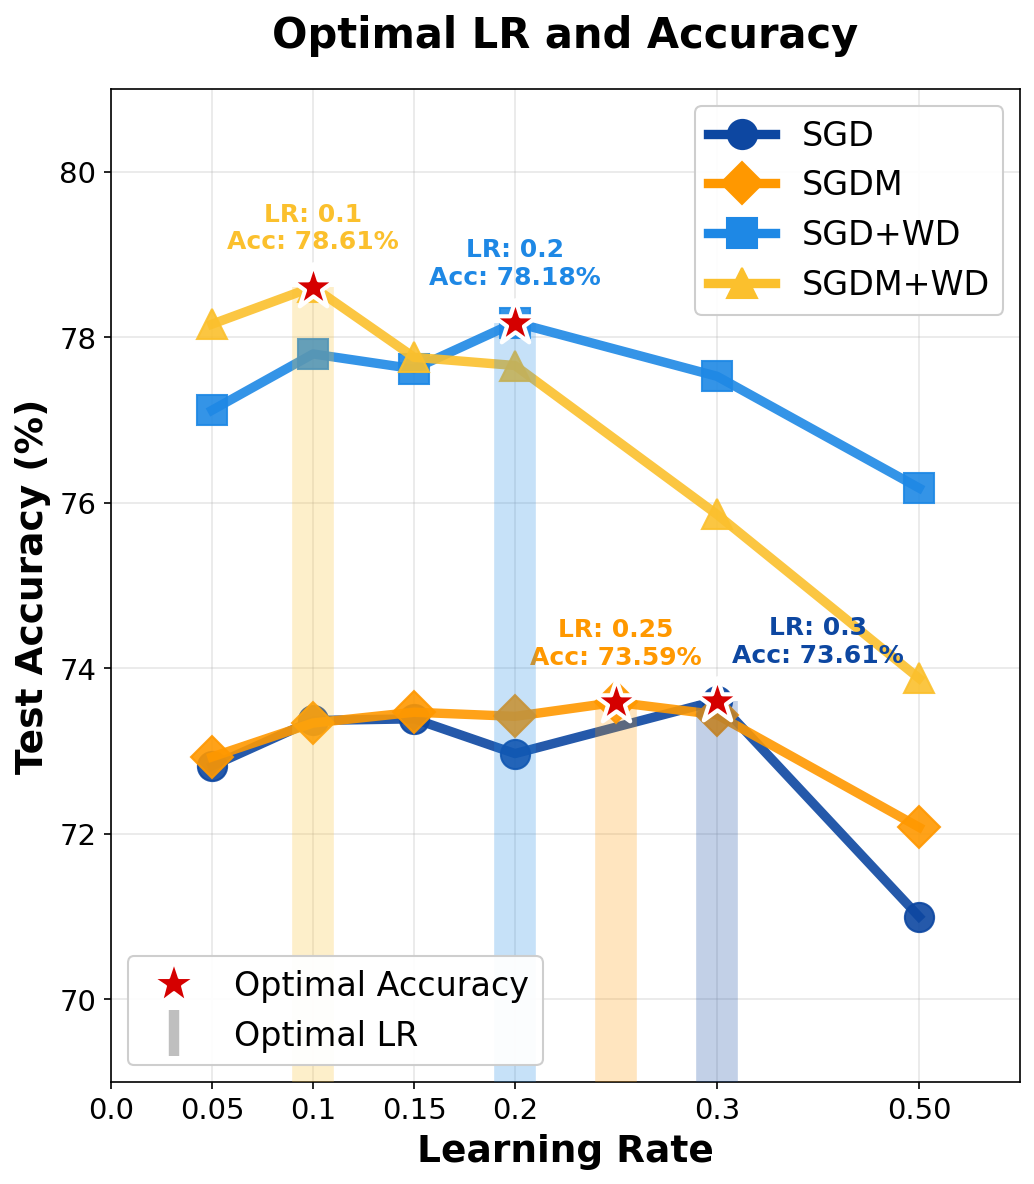
\includegraphics[width=0.98\linewidth]{figures/performance.jpg} 
    
    \vspace{-0.2cm} % 如果觉得标题离图片太远，可以用负值拉近一点
    
    \caption{The comparison of SGD, SGD-WD, SGDM, and SGDM-WD in optimal accuracy and corresponding learning rates.}
    \label{fig:performance}
    \vspace{-0.2cm} % 调整图片下方的空白，节省空间
\end{figure}

\textbf{Answer to Q1:} As demonstrated by Theorems \ref{thm:sgd}, \ref{thm:sgd-WD}, \ref{thm:sgdm} and \ref{thm:sgdm-WD}, weight decay not only enhances the generalization capability of base optimizers but also imposes new requirements on learning rate setting. Specifically, for the basic optimizer, the introduction of $\lambda$ significantly reduces the conditions of learning rate under optimal performance, which is also empirically verified, as shown in Figure \ref{fig:performance}. This prompts us to rethink the coupling between $\lambda$ and $\eta$.


\section{Generalization-Oriented Parameter Setting}
\begin{figure*}[t]
    \centering
    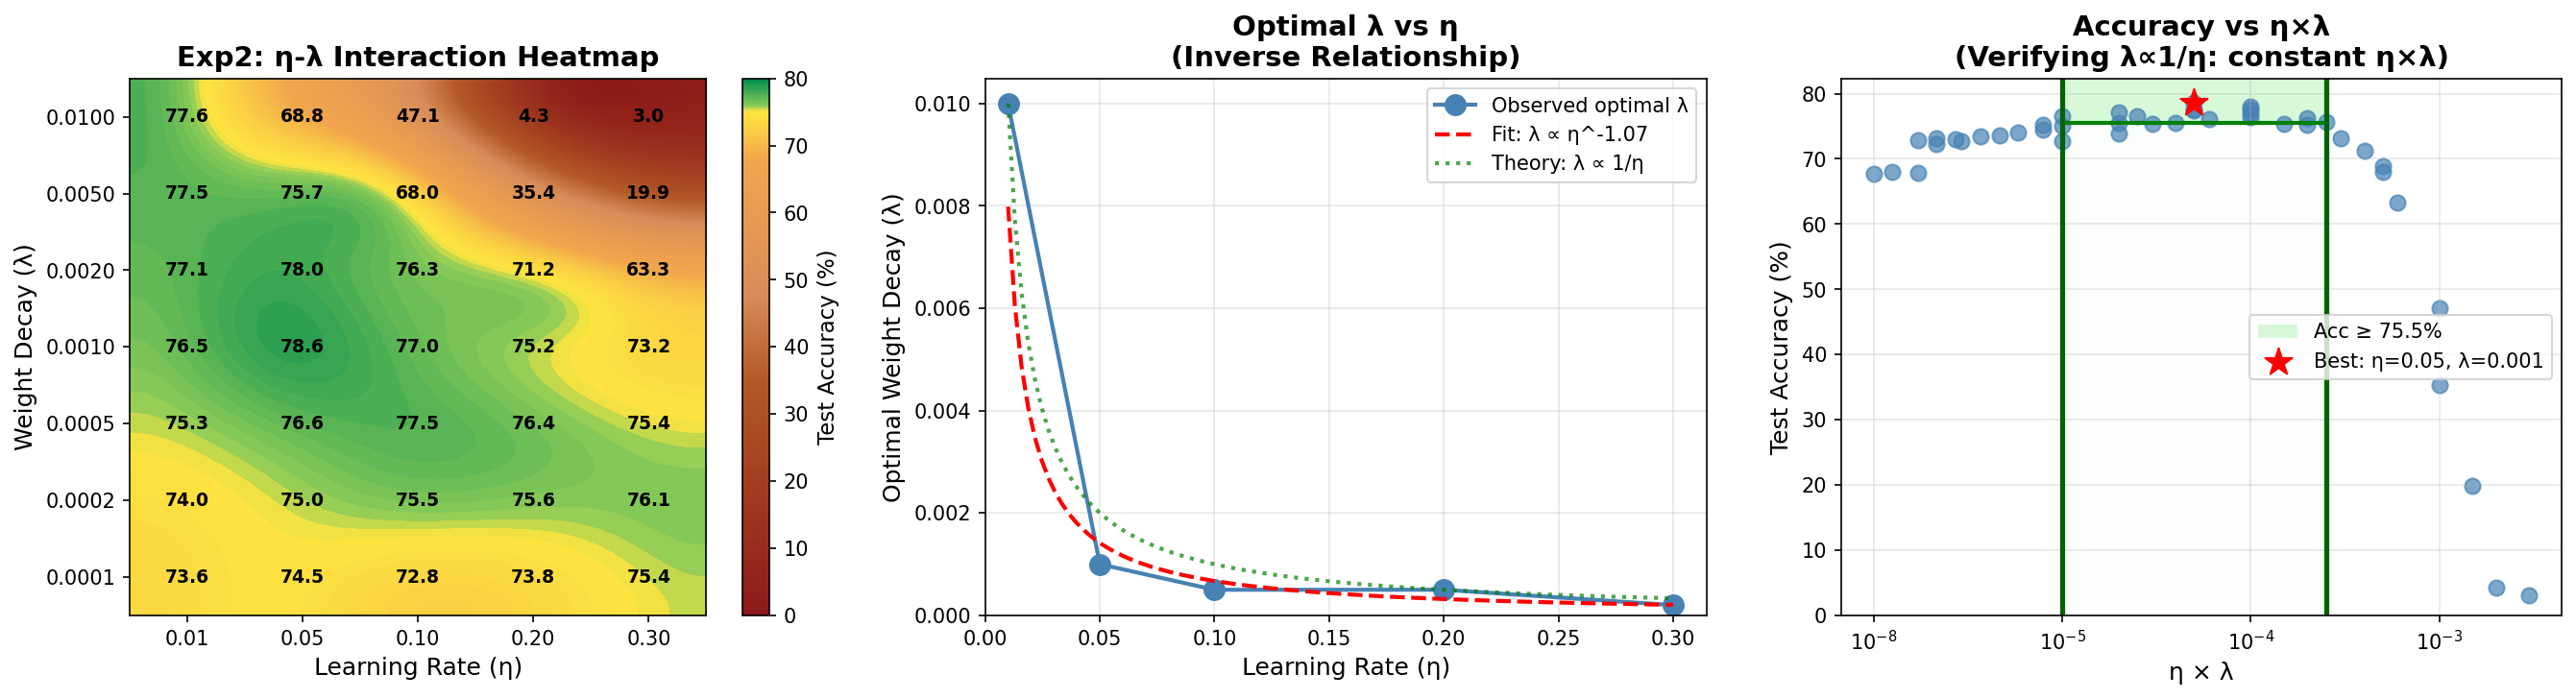
\includegraphics[width=\linewidth]{figures/WD and LR.jpg}
    \caption{Optimal test accuracy and corresponding learning rates for SGD, SGDM, SGD-WD, and SGDM-WD. Left: Learning rate versus weight decay, where each entry indicates the best test accuracy achieved for a given hyperparameter pair. Middle: The solid blue curve connects five observed points; the red dashed curve is fitted using five observations; the green dashed curve represents the theoretically predicted inverse relationship between parameters $\lambda$ and $\eta$. Right: Test accuracy plotted against the joint configuration of $\lambda$ and $\eta$.}
    \label{fig:WD and LR}
    \vspace{-0.8em} 
\end{figure*}

\begin{tcolorbox}
\textbf{Q2:} Can we derive a quantitative scaling Law via uniform stability theory that precisely reveals the intrinsic coupling mechanism between $\lambda$, $\eta$, $B$, and other parameters?
\end{tcolorbox}

\citet{wang2025setadamwsweightdecay} model AdamW as an Exponential Moving Average (EMA). Through formal analogy, they derived an explicit relationship among the $\lambda$, $\eta$, and $T$ as
\begin{equation}
 \lambda = \frac{1}{\eta T} ,   
\end{equation}
implying an inverse proportionality between the learning rate and weight decay when iterations $T$ are fixed. 

\textbf{Motivation:} Building on the "Regularization Equivalence" hypothesis proposed in this work, we seek to quantify the interplay between hyperparameters through the lens of Uniform Stability. Instead of treating hyperparameters in isolation, we postulate that SGD-WD and SWA should satisfy comparable stability constraints to achieve identical generalization. This theoretical alignment allows us to derive the implicit coupling relationship, laying the mathematical foundation for the scaling laws proposed in this work.

\subsection{Coupling of $\lambda$ and $\eta$}
We first present the generalized bound for the SWA.

\begin{lemma}{\rm (\citet[Theorem 4.1]{pmlr-v235-wang24bl})}\label{thm:SWA}
Assume that the loss function $F(\theta;z)$ is convex, Lipschitz and $L$-smooth for all given $z\in\mathcal{Z}$ with sizes $n$. Suppose we run WA with step sizes $\eta \leq \frac{2}{L}$ for $T$ steps, where each step samples $z_i$ from $\mathcal{Z}$ without replacement. Then, WA has uniform stability of
\begin{equation}
  \epsilon_{gen} = \mathbb{E}\vert F(\bar{\theta}_T;z)-F(\bar{\theta}^{\prime}_T;z)\vert \leq \frac{\eta G^2 T}{n}.
 \end{equation}
\end{lemma}

\begin{remark}
Theorem \ref{thm:SWA} shows that under the assumption of convexity, the generalization bound of SWA is half that of SGD, implying a significant improvement in generalization performance. This is a well-established result, and its detailed proof can be found in \cite{pmlr-v235-wang24bl,hardt2016train,xiao2022stability}. 
\end{remark}

By bridging the generalization bounds of SGD-WD (Theorem \ref{thm:sgd-WD}) and SWA (Theorem \ref{thm:SWA}) under the Regularization Equivalence hypothesis, we equate their stability constraints to obtain the following scaling relationship:
\begin{equation}\label{coupling:lamda}
\lambda \approx \frac{C}{\eta T} \implies \lambda \eta T \approx \text{Constant},
\end{equation}
where $C$ subsumes constant factors. It captures the dependency relationship between $\eta$ and $\lambda$ that must be followed to maintain system stability across varying training durations.

\begin{remark}
Eq.~\eqref{coupling:lamda} predicts that for a fixed iteration $T$, $\lambda$ must scale inversely with $\eta$. This theoretical derivation corroborates recent empirical findings in \cite{wang2025setadamwsweightdecay,bergsma2025powerlinesscalinglaws}. As visualized in the middle of Fig. \ref{fig:WD and LR}, our experimental data aligns well with this theoretical curve $1/x$, confirming that the heuristic alignment of stability bounds successfully captures the intrinsic coupling.
\end{remark}

\begin{remark}
Eq.~\eqref{coupling:lamda} suggests that $\eta$ and $\lambda$ play commensurate roles in the system. This implies that extreme concurrent configurations of these parameters will destabilize the training process. As demonstrated in the left and right of Figure \ref{fig:WD and LR}, the model attains optimal generalization only when the joint product of these hyperparameters (e.g., $\eta \cdot \lambda$) is maintained within an appropriate interval.
\end{remark}

 \subsection{Coupling of $\lambda$, $\eta$ and $B$}
To explicitly incorporate the batch size $B$, we rewrite the total iterations as $T = T_{epo} \cdot (n/B)$. Substituting this into Eq.~\eqref{coupling:lamda} yields the batch-dependent scaling law:
\begin{equation}\label{coupling:Batch}
\lambda \propto \frac{B}{\eta n T_{epo}}.
\end{equation}

\begin{figure*}[t]
    \centering
    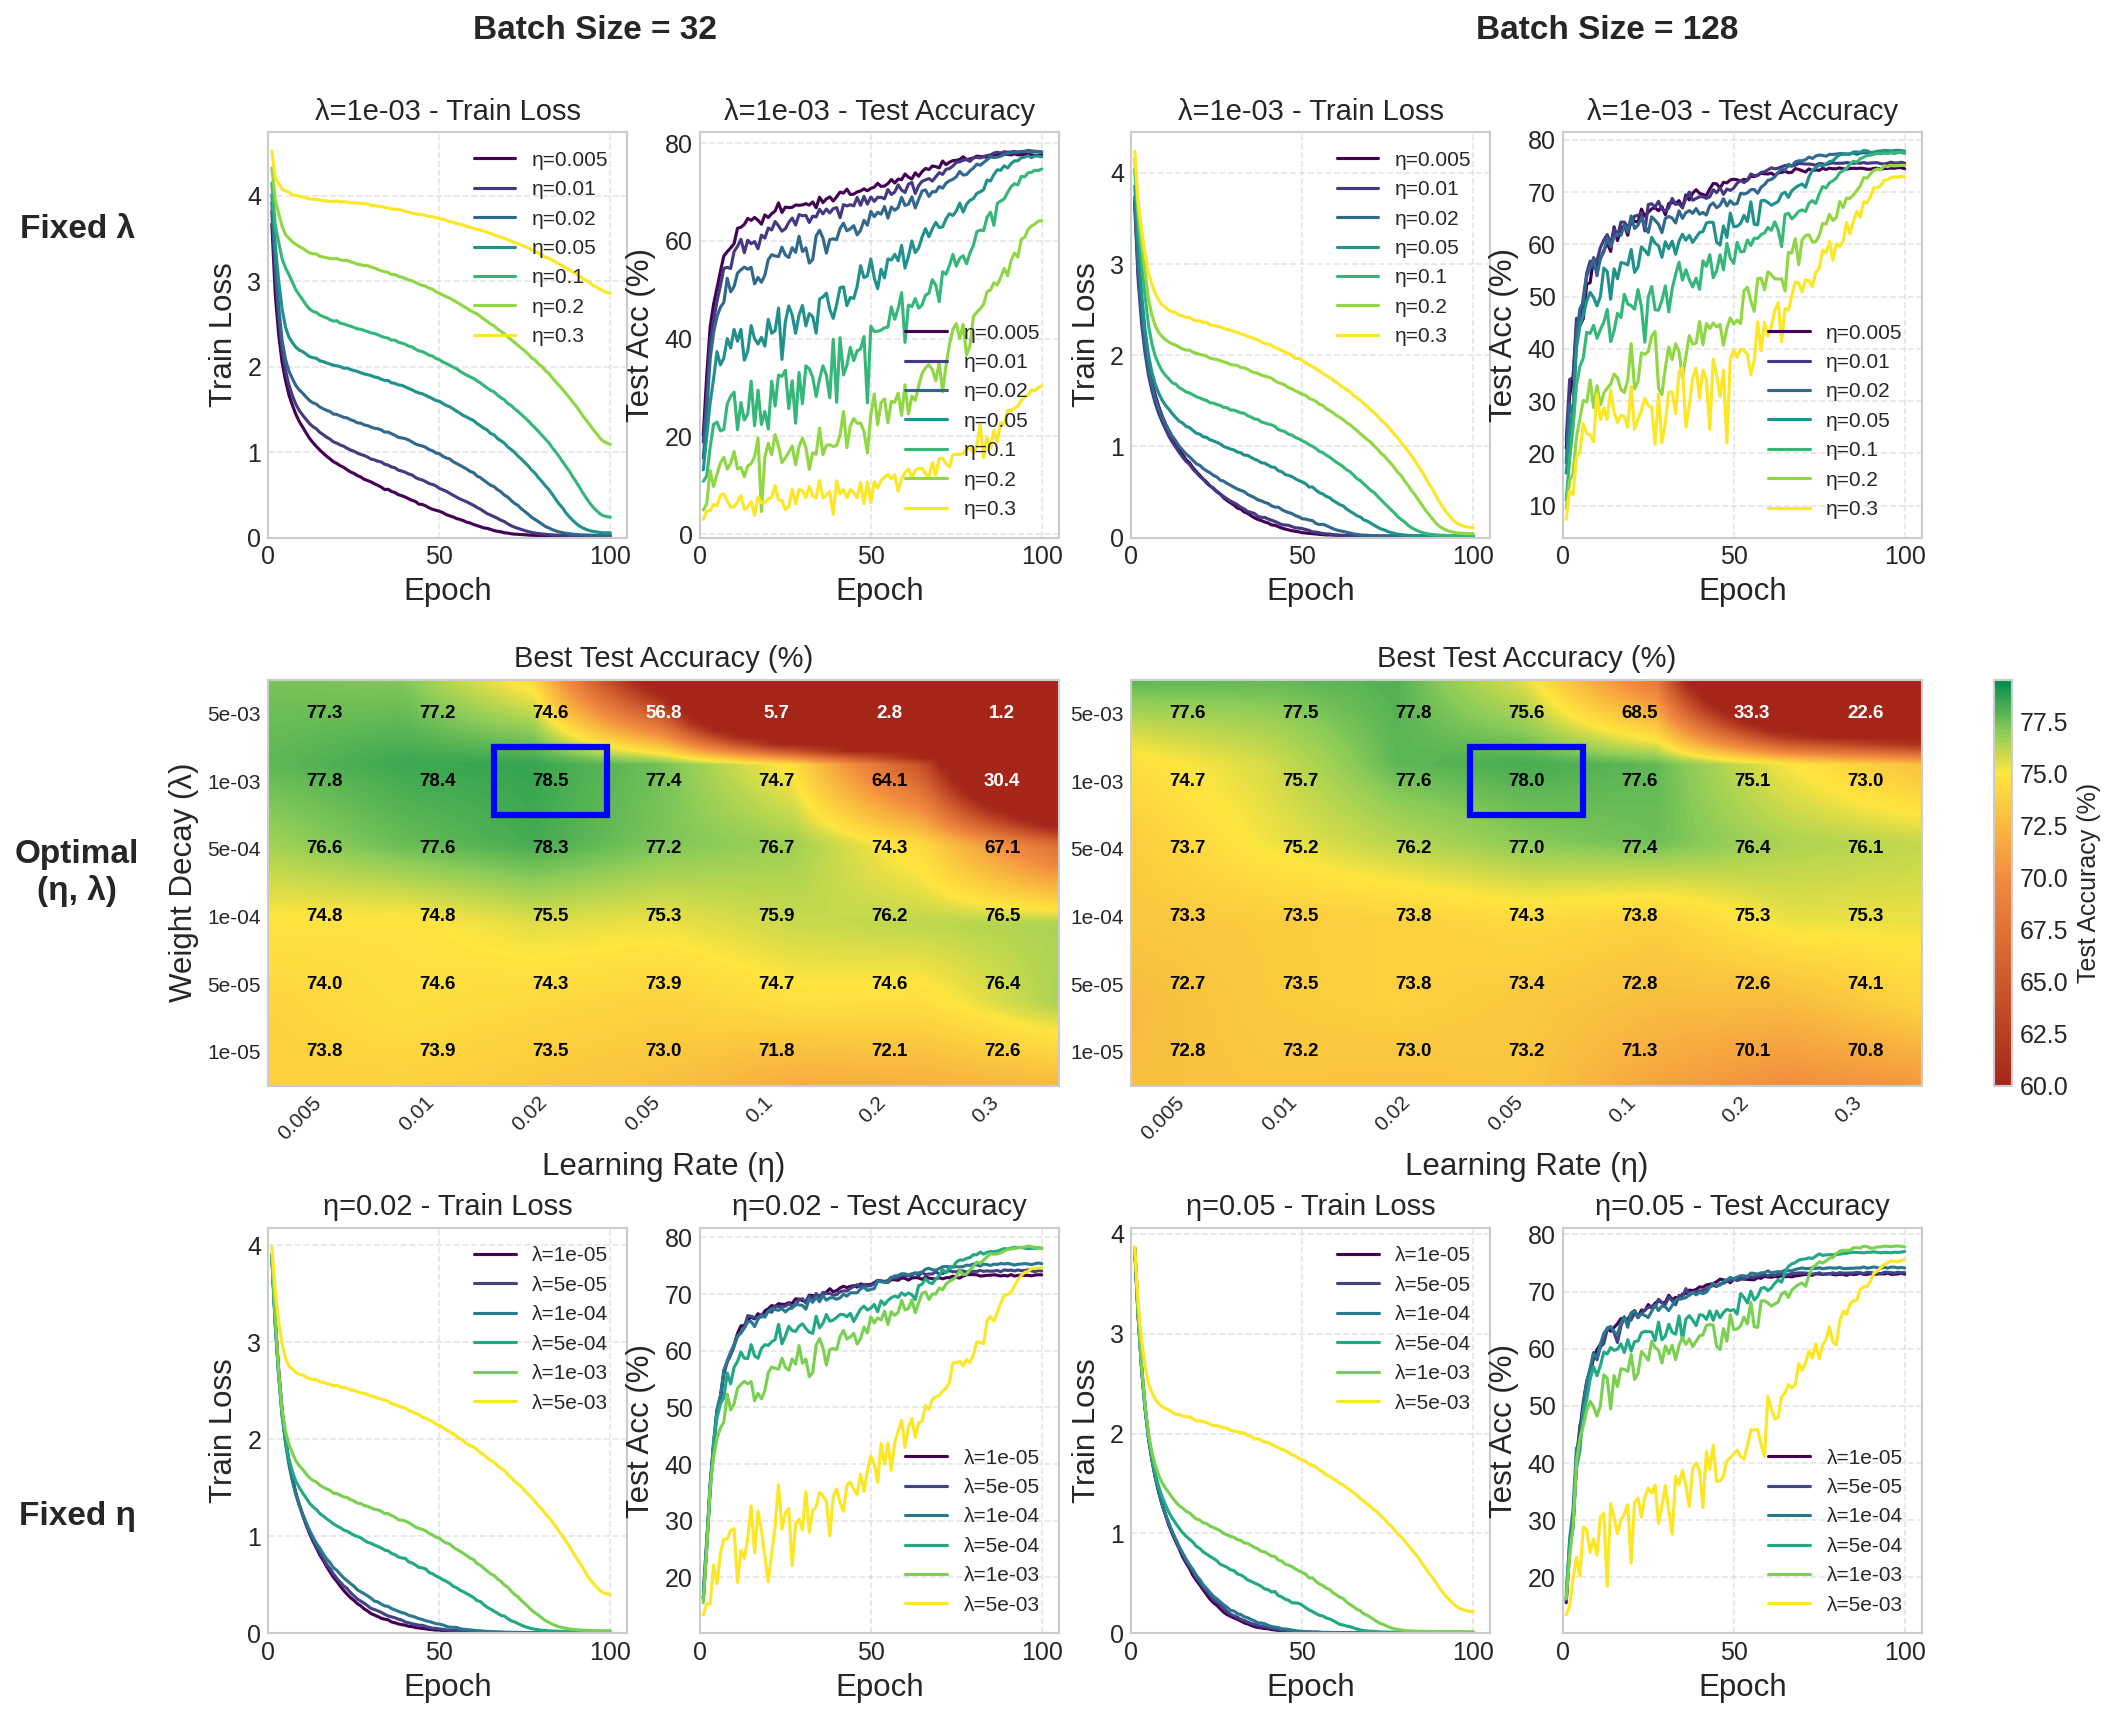
\includegraphics[width=\linewidth]{figures/batch.png}
    \caption{Coupling effects among hyperparameters at optimal performance after introducing batch size $B$. Top: For a fixed $\lambda$, the left and right subplots compare model performance across different $\eta$ with $B=32$ and $B=128$, respectively. Middle: Comparison of the optimal performance against the joint values of $\lambda\times\eta$ for $B=32$ (left) and $B=128$ (right). Bottom: For a fixed $\eta$, the left and right subplots compare model performance across different weight decay values $\lambda$ with $B=32$ and $B=128$, respectively.}
    \label{fig:batch}
    \vspace{-1em}  
\end{figure*}
 
\begin{remark}
Eq.~\eqref{coupling:Batch} reveals a fundamental compensation mechanism between explicit and implicit regularization. Small-batch training introduces significant gradient noise, acting as a strong implicit regularizer. As $B$ increases, this noise diminishes, creating a "regularization deficit." Consequently, to conserve total stability, the explicit weight decay $\lambda$ (and learning rate $\eta$) must be scaled up proportionally to compensate. This theoretical insight perfectly matches the empirical trends in Figure~\ref{fig:batch}, where increasing $B$ from 32 to 128 necessitates shifting the optimal $\lambda$ from $5\text{e-}4$ to $1\text{e-}3$.
\end{remark}

\textbf{Answer to Q2:} As shown in Eq. \ref{coupling:lamda} and \ref{coupling:Batch}, $\lambda$ acts as a counterweight to $\eta \cdot T$, requiring an inverse adjustment to maintain equilibrium, as validated by experience in Figure \ref{fig:WD and LR}. When Batch Size $B$ is introduced, it acts as a scaling factor: larger batches reduce implicit noise, necessitating a proportional increase in the joint magnitude of $\lambda$ and $\eta$ to preserve the stability, as shown in the Figure \ref{fig:batch} and Figure \ref{fig:LLM1} (the latter verified using LLM).


% \begin{remark}
% This scaling law offers actionable guidance for constrained scenarios. In resource-limited regimes (small $B$), one should reduce the joint product $\lambda \cdot \eta$ to prevent over-regularization (since noise is already high). Conversely, in throughput-prioritized regimes (large $B$), one can explore a larger $\lambda \cdot \eta$ product to accelerate convergence without sacrificing stability, consistent with the results in Figure \ref{fig:batch} (Middle).
% \end{remark}

% \begin{remark}
% Under practical constraints, such as limited computational resources where only small batch sizes are feasible, the proposed scaling law suggests selecting $\lambda\times\eta$ at lower values to ensure better test performance. In contrast, when computational resources are sufficient and efficiency is prioritized, a larger $\lambda\times\eta$ can be explored, which is consistent with the trend shown in the middle of Figure \ref{fig:batch}.
% \end{remark}

